\subsection{\nameref*{subsec:LFSRs} Sequences and Extension Fields}\label{LFSR_Sequences_Extension_Fields}
Let $\pi(x)$ be an \nameref{def:Irreducible_Polynomial} \nameref{def:Polynomial} over \TextFiniteMathField{F}{q}{} and assume its coefficients are
\begin{equation}\label{eq:Reciprocal_Connection_Polynomial}
  \pi(x) = x^{L} + c_{1}x^{L-1} + \cdots + c_{L}
\end{equation}
This means that $\pi(x)$ is the \emph{reciprocal} \nameref{def:Polynomial} of the \nameref{def:Connection_Polynomial} $C(D)$.

We can construct an \nameref{rmk:Extension_Field} \TextFiniteMathField{F}{q}{L} through $\pi(\alpha) = 0$.
The term $\beta$ from \TextFiniteMathField{F}{q}{} can be expressed in a \nameref{def:Polynomial} basis as
\begin{equation}\label{eq:Extension_Field-Beta}
  \beta = \beta_{0} + \beta_{1}\alpha^{1} + b_{2}\alpha^{2} + \cdots + \beta_{L-1} + \alpha^{L-1}
\end{equation}
where $\beta_{0}, \beta_{1}, \ldots, \beta_{L-1} \in \FiniteMathField{F}{q}{}$.

If we multiply \Cref{eq:Extension_Field-Beta} by $\alpha$, we get
\begin{equation*}
  \alpha\beta = \beta_{0}\alpha + \beta_{1}\alpha^{2} + \cdots + \beta_{L-1}\alpha^{L}
\end{equation*}
Now, we can reduce the $\alpha^{L}$ according to the $\pi(\alpha)=0$ relation we found earlier.
This gives us
\begin{equation}\label{eq:LFSR_Galois_Equation}
  \alpha\beta = -c_{L}\beta_{L-1} + \left( \beta_{0} - c_{L-1}\beta_{L-1} \right) \alpha + \cdots + \left( \beta_{L-2} - c_{1}\beta_{L-1} \right) \alpha^{L-1}
\end{equation}

\begin{figure}[h!]
  \centering
  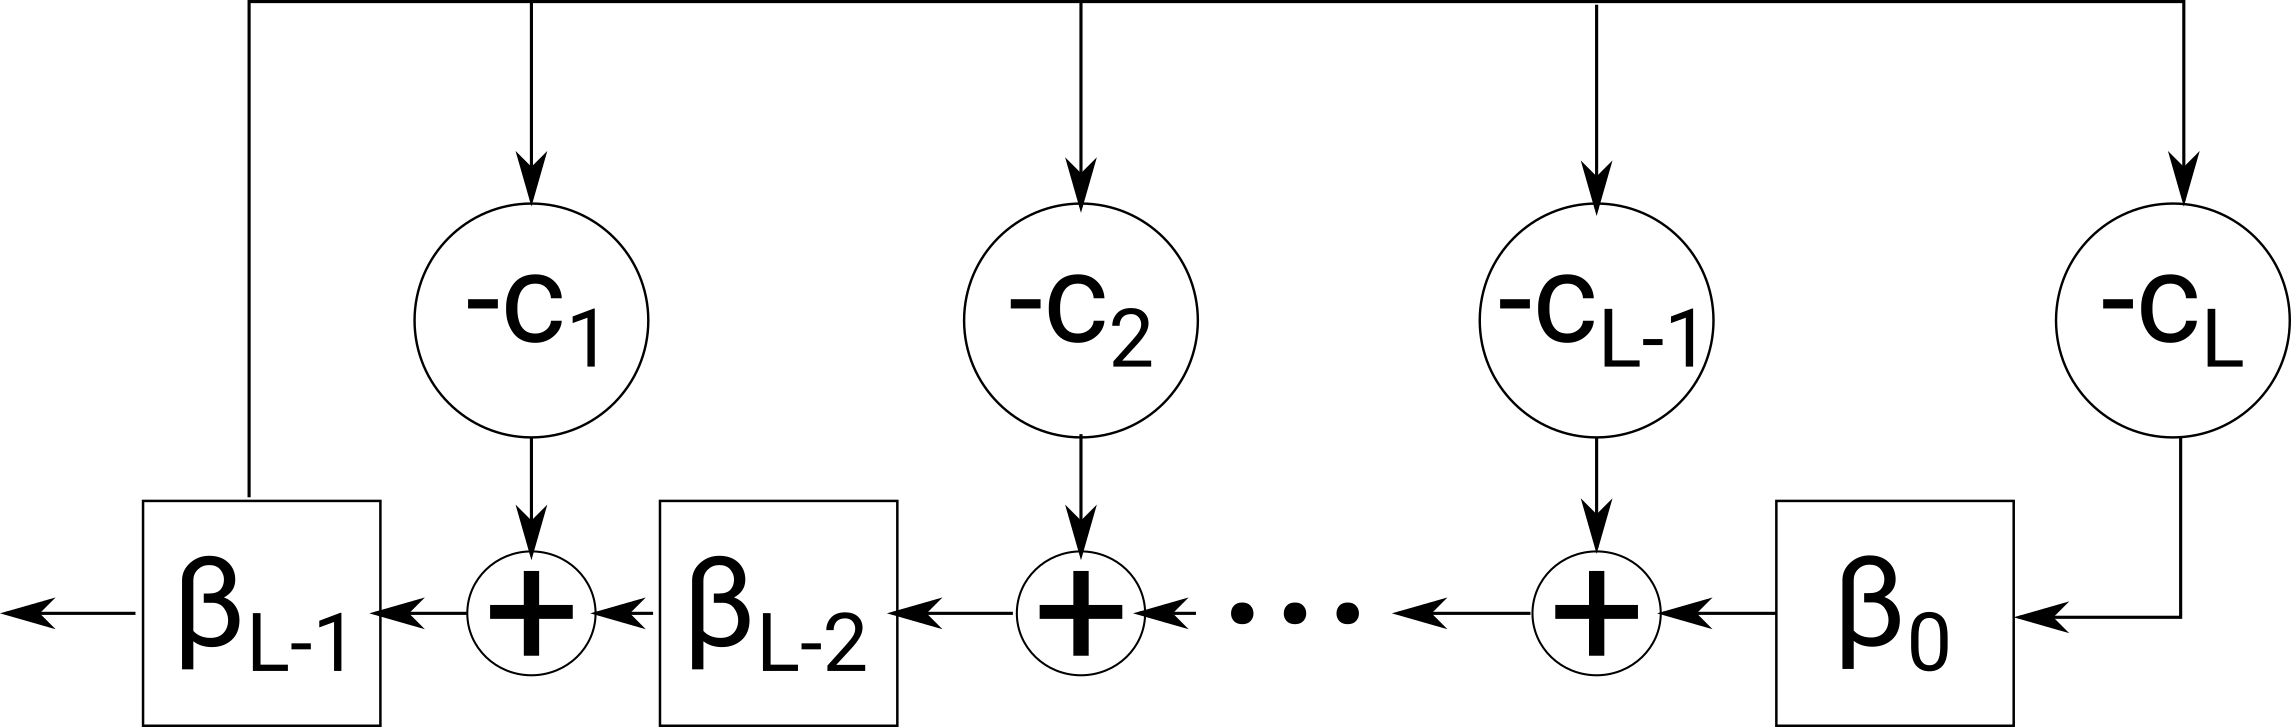
\includegraphics[scale=0.5]{./Linear_Feedback_Shift_Register-Galois.png}
  \caption{\nameref{def:LFSR} in Galois Form}
  \label{fig:LFSR_Galois}
\end{figure}

We can check that this form, the \emph{Galois Form} of this \nameref{def:LFSR} is the same as the other.
\begin{equation*}
  s_{j} = -c_{1}s_{j-1} - c_{2}s_{j-2} - \cdots - c_{L}s_{j-L}
\end{equation*}
when $j \geq L$.
Also,
\begin{equation*}
  p_{0} = s_{0}, p_{1} = s_{1} + c_{1}s_{0}, \ldots
\end{equation*}
where $p_{0}, p_{1}, \ldots, p_{L-1}$ is the initial state of the \nameref{def:LFSR} in its Galois Form.

\begin{blackbox}
  The set of \nameref{def:LFSR} sequences, when $C(D)$ is \nameref{def:Irreducible_Polynomial}, is exactly the set of sequences possible to produce by the implmentation of multiplication of an element $\beta$ by the fixed element $\alpha$ in \TextFiniteMathField{F}{q}{L}.
  \tcblower{}
  For a specific sequence specified as $S(D) = \frac{P(D)}{C(D)}$, the initial state if the first $L$ symbols, whereas the same sequence is produced in \Cref{fig:LFSR_Galois} if the initial state is $p_{0}, p_{1}, \ldots, p_{L-1}$.
\end{blackbox}

\subsubsection{Properties of \nameref*{subsec:LFSRs}}\label{subsubsec:LFSR_Properties}
\begin{propertylist}
\item A sequence $\mathbf{s} = \ldots, s_{0}, s_{1}, \ldots$ is called \emph{periodic} if there is a positive integer $T$ such that $s_{i} = s_{i+T} \: \forall i \geq 0$.
\item The \emph{period} is the least such positive integer $T$ for which $s_{i} = s_{i+T} \: \forall i \geq 0$
\item The \nameref{def:LFSR} state runs through different values. The initial state will appear again after visiting a number of states.
  If $\Degree \bigl( C(D) \bigr) = L$, the period of a sequence is the same as the number of different states visited, before returning to the initial state.
\item If $C(D)$ is \nameref{def:Irreducible_Polynomial}, the state corresponds to an element in \TextFiniteMathField{F}{q}{L}, call it $\beta$.
\item The sequence of diferent states that we are entering is
  \begin{equation*}
    \beta, \alpha\beta, \alpha^{2}\beta , \ldots, \alpha^{T-1}\beta, \left( \alpha^{T}\beta = \beta \right)
  \end{equation*}
  where $T$ is the \nameref{def:Element_Order} of $\alpha$
\end{propertylist}

\begin{definition}[$m$-Sequence]\label{def:M_Sequence}
  An \emph{$m$-sequence} is one where $\alpha$ is a \nameref{def:Polynomial_Ring_Properties-Primitive_Element}.
  This means we go through all $q^{L}-1$ states, where $\ElementOrder(\alpha) = q^{L}-1$.
  These will only appear if and only if the \nameref{def:Polynomial} $\pi(x)$ is a \nameref{def:Polynomial_Ring_Properties-Primitive_Element}.
  A $\pi(x)$ being \nameref{def:Irreducible_Polynomial} is not enough, it \textbf{must} also be \nameref{def:Polynomial_Ring_Properties-Primitive_Element}.
\end{definition}

A periodic and causal sequence, we denoted ${\left[ s_{0}, s_{1}, \ldots, s_{T-1} \right]}^{\infty}$.
This is equivalent to
\begin{equation*}
  s_{0}, s_{1}, \ldots, s_{T-1}, s_{0}, s_{1}, \ldots, s_{T-1}, s_{0}, \ldots
\end{equation*}
where $s_{i} \in \FiniteMathField{F}{q}{}, i = 0, 1, \ldots, T-1$

\begin{definition}[Polynomial Period]\label{def:Polynomial_Period}
  The \emph{period of a \nameref{def:Polynomial}} $C(D)$ is the least positive integer $T$ such that $C(D) \Divides \left( 1-D^{T} \right)$.

  This is calculated by dividing 1 by $C(D)$ and continuing until you receive a remainder of the form $1\cdot D^{N}$.
  The remainder \textbf{MUST} have the coefficient of 1.
  And the value of $T=N$.
\end{definition}

\begin{example}[Lecture 9, Example 4.6]{Polynomial Period}
  Calculate the period of the \nameref{def:Polynomial} $C(D) = 3 + D^{2}$ in \TextFiniteMathField{F}{5}{}?
  \tcblower{}
  Start by dividing 1 by $C(D)$.

  \begin{equation*}
    \frac{1}{3+D^{2}} = 2 + D^{2} + 3D^{4} + 4D^{6}
  \end{equation*}
  with a remainder of $1D^{8}$.

  Thus, the period of $C(D) = 3+D^{2}$ is $T=8$.
  We can check this by making sure the remainder of the division is 0, with
  \begin{center}
    \polylongdiv{1-D^{8}}{3+D^{2}}
  \end{center}
  and it is, so we found the right answer.
\end{example}

\begin{theorem}\label{thm:GCD_Connection_Polynomial_S_Sequence}
  If $\gcd \bigl( C(D), P(D) \bigr) = 1$, then the \nameref{def:Connection_Polynomial} $C(D)$ and the sequence $\mathbf{s}$ with \nameref{def:D_Transform}
  \begin{equation*}
    S(D) = \frac{P(D)}{C(D)}
  \end{equation*}
  have the same period, the period of $\mathbf{s}$ is the same as the \nameref{def:Polynomial_Period} $C(D)$.
\end{theorem}
\begin{itemize}[noitemsep]
\item This $C(D)$ gives the shortest \nameref{def:LFSR} generating $\mathbf{s}$.
\item Any other $C(D)$ generating $\mathbf{s}$ must be a multiple of $C(D)$.
\end{itemize}

\begin{theorem}\label{thm:Adding_D_Transform_Sequence}
  If the 2 sequences $\mathbf{s}_{A}$ and $\mathbf{s}_{B}$, with period $T_{A}$ and $T_{B}$ have \nameref{def:D_Transform}s
  \begin{align*}
    S_{A}(D) &= \frac{P_{A}(D)}{C_{A}(D)} & S_{B}(D) &= \frac{P_{B}(D)}{C_{B}(D)}
  \end{align*}
  then the sum of the sequences $\mathbf{s} = \mathbf{s}_{A} = \mathbf{s}_{B}$ has a \nameref{def:D_Transform}
  \begin{equation}\label{eq:Add_D_Transform_Sequences}
    S(D) = S_{A}(D) + S_{B}(D)
  \end{equation}
  and the shared period is
  \begin{equation}\label{eq:Period_Add_D_Transform_Sequences}
    \lcm \left( T_{A}, T_{B} \right)
  \end{equation}

  This all happens under the assumptions:
  \begin{itemize}[noitemsep]
  \item $\gcd \bigl( P_{A}(D), C_{A}(D) \bigr) = 1$
  \item $\gcd \bigl( P_{B}(D), C_{B}(D) \bigr) = 1$
  \item $\gcd \bigl( C_{A}(D), C_{B}(D) \bigr) = 1$
  \end{itemize}
\end{theorem}

\begin{example}[Lecture 9, Example 4.7]{Shortest LFSR Sequence}
  Given the sequence ${[1, 0, 1, 0, 0, 1, 1]}^{\infty}$ in \TextFiniteMathField{F}{2}{}, what is the shortest \nameref{def:LFSR} that can produce this sequence?
  \tcblower{}
  Start by finding the general case of this sequence, in a \nameref{def:D_Transform}ed state.
  \begin{equation*}
    S(D) = \frac{1+D^{2}+D^{5}+D^{6}}{1+D^{7}}
  \end{equation*}
  The numerator is drawn from the given sequence.
  The denominator is found from the length of the period.
  However, this is not the shortest \nameref{def:LFSR} possible to generate this sequence.

  If we find a common factor, we can simplify this \nameref{def:LFSR}.
  \begin{equation*}
    \gcd(1+D^{2}+D^{5}+D^{6}, 1+D^{7})
  \end{equation*}
  We solve this with the \nameref{def:Polynomial_Euclidean_Algorithm}.

  \begin{align*}
    1+D^{7} &= q(D) \left( 1+D^{2}+D^{5}+D^{6} \right) + r(D) \\
    &= \left( D+1 \right) \left( 1+D^{2}+D^{5}+D^{6} \right) + \left( D^{5}+D^{3}+D^{2}+D \right) \\
  \end{align*}
  Since the remainder is not 0, we continue reducing.
  \begin{align*}
    \left( 1+D^{2}+D^{5}+D^{6} \right) &= q(D) \left( D^{5}+D^{3}+D^{2}+D \right) + r(D) \\
                                       &= \left( D+1 \right) \left( D^{5}+D^{3}+D^{2}+D \right) + \left( D^{4}+D^{2}+D+1 \right) \\
    \left( D^{5}+D^{3}+D^{2}+D \right) &= q(D) \left( D^{4}+D^{2}+D+1 \right) + r(D) \\
    &= (D) \left( D^{4}+D^{2}+D+1 \right) + 0 \\
  \end{align*}
  So, the $\gcd(1+D^{2}+D^{5}+D^{6}, 1+D^{7}) = D^{4}+D^{2}+D+1$.

  Now we factor that value out of the $S(D)$ fraction, and reduce it out.
  \begin{align*}
    S(D) &= \frac{\left( D^{4}+D^{2}+D+1 \right) \left( D^{2}+D+1 \right)}{\left( D^{4}+D^{2}+D+1 \right) \left( D^{3}+D+1\right)} \\
    &= \frac{\left( D^{2}+D+1 \right)}{\left( D^{3}+D+1\right)}
  \end{align*}

  Thus, the shortest \nameref{def:LFSR} for the given sequence has a \nameref{def:Connection_Polynomial} of $C(D) = D^{3}+D+1$, with an initial state \nameref{def:D_Transform} equation of $P(D) = D^{2}+D+1$.
\end{example}

%%% Local Variables:
%%% mode: latex
%%% TeX-master: "../../EDIN01-Cryptography-Reference_Sheet"
%%% End:
